\documentclass[11pt,a4paper]{article}
\usepackage[a4paper,margin=24mm]{geometry}
\usepackage{amsmath,amssymb,amsthm}
\usepackage{booktabs,tabularx,longtable}
\usepackage{graphicx}
\usepackage[colorlinks=true,linkcolor=blue,urlcolor=blue]{hyperref}
\usepackage[T1]{fontenc}
\usepackage{lmodern}
\usepackage{microtype}
\sloppy
\setlength{\parskip}{4pt}
\renewcommand{\Re}{\operatorname{Re}}
\title{Referee report\\[3pt]\large ``The Quasi-Riemann Hypothesis: A Zero-Free Half-Plane $\Re s>7/8$''\\
\normalsize (openai/math, commit \texttt{adc7f1241b42}, preprint dated 30 September 2026)}
\author{Independent verification report}
\date{7 October 2026}
\begin{document}
\maketitle

\section{Summary of the submission}
The preprint claims that every Dirichlet $L$-function, including $\zeta(s)$, and every finite-order Hecke
$L$-function over $F=\mathbb Q(\sqrt{-3})$ has no zero in $\Re s>7/8$ (principal pole at $s=1$ excepted).
The argument is a family-wide bootstrap. Let $\beta_*$ be the supremum of the real parts of the zeros of all
primitive finite-order Hecke $L$-functions over $F$. If $\beta_*>\sigma_0$, a probe $J_\eta(Z)$ built from
cubic-theta (Kubota--Patterson) coefficients averaged against sextic residue characters is bounded directly
(the \emph{low} estimate, via cubic reflection and large sieves). The same probe is compared, after Poisson
summation, with the Mellin signal of $1/L(s,\eta)$ (the \emph{high} estimate). The non-principal Poisson rows
are Hecke twists inside the same family, whose zeros satisfy $\Re\rho\le\beta_*$; rows carrying zeros are
counted by a zero detector together with sextic large-sieve and moment estimates. A Landau-type continuation
principle (Proposition~2.1) then contradicts the definition of $\beta_*$. Part~I gives $11/12$, and Part~II
bootstraps from it to $7/8$. A Lean~4 formalization of the $\zeta$ and Dirichlet statements accompanies the
preprint.

\section{Overall assessment}
\textbf{Verdict.} The main theorem is correct for $\zeta$ and for all Dirichlet $L$-functions. I rebuilt
the accompanying Lean~4 formalization locally: 2{,}924 modules, no errors. The resulting theorem
\texttt{OAI.riemannZeta\_ne\_zero\_of\_seven\_eighths\_lt\_re}, whose type matches the comparator challenge
verbatim, depends only on the standard axioms \texttt{propext}, \texttt{Classical.choice} and
\texttt{Quot.sound}. The remaining trust base is the Lean kernel, the official Mathlib build cache, and
Mathlib's definitions of \texttt{riemannZeta} and \texttt{DirichletCharacter.LFunction}.


I found no structural defect that would refute the argument on general grounds, and no error in any part I
checked in full. The portions I verified by hand or by exact computer algebra are the continuation criterion,
the Hecke-to-Dirichlet transfer, the exponent bookkeeping of Section~20, and the endpoint certificate
(Lemma~20.2). The technically heaviest parts I did \emph{not} verify by hand: Proposition~5.1, Lemma~9.1,
Propositions~9.2 and~19.2, and Sections~17--18, about $10^4$ lines of \TeX. For these, the evidence of
correctness is the formal verification reported in Section~\ref{sec:lean}, which certifies the theorem but
not the prose argument line by line.

\section{What was checked}
\begin{enumerate}
\item \textbf{Provenance.} The repository, PDF (199~pp.), \TeX{} source (16{,}677 lines) and Lean sources were
  fetched through the GitHub API, and SHA-256 hashes were recorded.
\item \textbf{Structure.} 67 numbered statements were extracted from the \TeX{} labels and references. The
  section-level citation graph is acyclic; all 11 forward references are announcements of later proofs.
\item \textbf{Barrier tests.}
  \begin{itemize}
  \item \emph{Euler product.} The argument uses Euler products essentially: through the local Euler identity
    (Lemma~7.x, \texttt{lem:local-euler}), through M\"obius coefficients in the inverse detector polynomials,
    and through closure of the family under twisting. It therefore does not apply to the Davenport--Heilbronn
    function. We re-computed that function's off-line zero $0.808517+85.699348i$.
  \item \emph{Single zero versus density.} The target zero is never counted. It enters through the size of the
    Mellin signal of $1/L$, and density-type counts are used only for the other rows. This is a legitimate use
    of density estimates.
  \item \emph{Uniformity.} All exponent margins are fixed before the target: $m_{\rm lo}=\Delta$,
    $m_{\rm hi}=\tfrac{51}{64}\Delta$, $m_{\rm small}=63/800$, $m_w=23/960$, $m_z=13/9600$, and $\kappa_P$.
  \item \emph{Consistency.} The consequences (no Landau--Siegel zeros in $(7/8,1)$, Vinogradov's least
    non-residue conjecture via Bhargava--Ivanyos--Mittal--Saxena) contradict no known theorem or numerical data.
  \end{itemize}
\item \textbf{Exact arithmetic.} 66 explicit identities and inequalities were verified with \texttt{sympy}
  and \texttt{mpmath}; all pass. They include the boundary identity
  $C_{\rm II}(s)=l_x/2+s-1+h/6=s-11/16$, the completed-square certificate of Lemma~20.2, and every rational
  constant in Section~20. A $401\times401$ grid gives $\min(-E_*)=2.28\times10^{-4}$, about twice the
  certified $49/440640$.
\end{enumerate}

\begin{figure}[h]
\centering
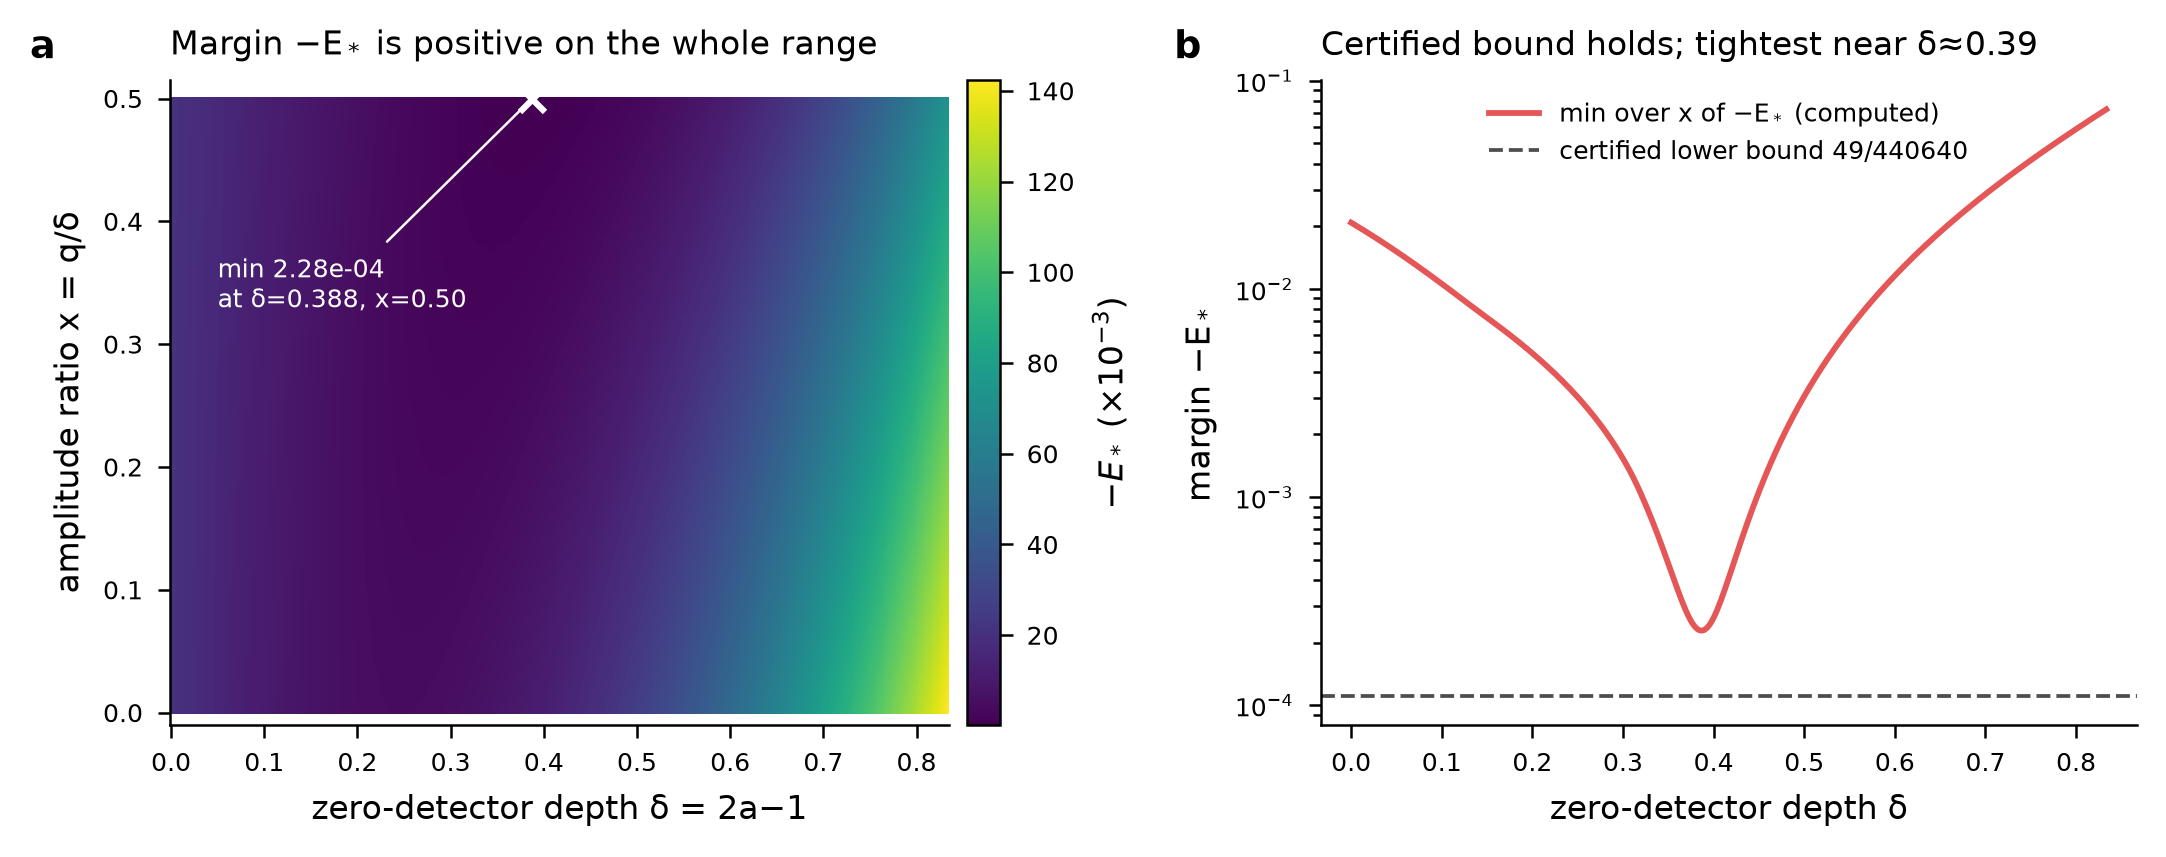
\includegraphics[width=\textwidth]{../figures/fig_endpoint_certificate.png}
\caption{Lemma 20.2. (a) The margin $-E_*(\delta,x)$ over the full parameter range. (b) Its minimum over $x$
against the certified lower bound $49/440640$ (dashed). The certificate holds everywhere and is tightest near
$\delta\approx0.39$, $x=1/2$.}
\end{figure}

\section{Formal verification}\label{sec:lean}
\begin{itemize}
\item \textbf{Statement fidelity.} The challenge file states
  \texttt{theorem riemannZeta\_ne\_zero\_of\_seven\_eighths\_lt\_re \{s : \ensuremath{\mathbb{C}}\} (hs : (7 / 8 : \ensuremath{\mathbb{R}}) < s.re) :
  riemannZeta s \ensuremath{\neq} 0} using Mathlib definitions only. A verbatim copy of this statement was proved from the
  solution theorem, which confirms the type match; the same holds for the Dirichlet statement. Mathlib's junk
  value $\texttt{riemannZeta}\,1=(\gamma-\log4\pi)/2\neq0$ is consistent with the statement.
\item \textbf{Build.} Lean 4.34.1 (official \texttt{darwin\_aarch64} release) with Mathlib \texttt{d13f23b}
  (official cache), PrimeNumberTheoremAnd \texttt{c39a751} and rellich-kondrachov \texttt{70f85d4} (with the
  repository's compatibility patches). The command
  \texttt{lake build OAI.NumberTheory.DirichletL.Nonvanishing} completed 7{,}061 jobs, including local
  elaboration and kernel checking of all 2{,}924 OAI modules, with no errors and no \texttt{sorry} warnings
  (252~min on 8~cores / 16\,GB).
\item \textbf{Axioms.} \texttt{\#print axioms} gives \texttt{[propext, Classical.choice, Quot.sound]} for both
  the $\zeta$ and the Dirichlet theorem.
\item \textbf{Static scan.} The OAI closure contains no occurrence of \texttt{sorry}, \texttt{axiom},
  \texttt{native\_decide}, \texttt{implemented\_by}, \texttt{extern}, \texttt{unsafe}, \texttt{opaque},
  \texttt{run\_cmd}, \texttt{elab}, \texttt{macro\_rules}, \texttt{initialize}, \texttt{skipKernelTC} or
  \texttt{addDecl}. PrimeNumberTheoremAnd contains two test axioms in a tactic file; the axiom output shows
  that the theorem does not use them.
\item \textbf{Independent kernel replay.} Time-boxed. A full \texttt{leanchecker} replay of all 2{,}924 OAI modules was stopped after about 60 minutes without completing; no error had been reported. The replay of the two final modules (\texttt{Nonvanishing} and \texttt{FinalAssemblyUnconditional}) completed without error. In the ordinary build, the kernel already checks every declaration as it is added.
\item \textbf{Not covered.} The Hecke challenge, which uses local definitions, was not built, and no mapping
  from the paper's numbered statements to Lean declarations is provided.
\end{itemize}


\section{Major comments}
\begin{enumerate}
\item \textbf{Where the boundary comes from.} The low estimate and the Mellin normalization give exactly
  $\sigma_0=1-h/6+b/12$, which yields $11/12$ for $(h,b)=(1/2,0)$ and $7/8$ for $(13/16,1/8)$. Several stated
  hypotheses stop exactly at $7/8$:
  \begin{itemize}
  \item \texttt{lem:bin-contour-accounting} assumes $\sigma_0\in[7/8,1)$;
  \item the second region of \texttt{lem:local-euler} requires $\Re x\ge7/8$;
  \item \texttt{lem:plain} assumes $\kappa\ge3/4$.
  \end{itemize}
  The authors should say explicitly that $7/8$ is (nearly) optimal for this parametrization. Our re-optimization
  of the Section~20 constraints gives $0.87496$; see Section~\ref{sec:barrier}.
\item \textbf{Hecke statement.} The Lean challenge for Hecke $L$-functions over $\mathbb Q(\sqrt{-3})$ uses
  definitions local to the challenge file. Their faithfulness to the paper's $L_F(s,\eta)$ should be audited
  independently. The $\zeta$ and Dirichlet challenges use only Mathlib definitions.
\item \textbf{Dependency patches.} The build applies large compatibility patches to third-party packages
  (e.g.\ 2\,MB for PrimeNumberTheoremAnd). Soundness is protected by the axiom check, but the authors should
  state what the patches change.
\end{enumerate}

\section{Minor comments}
\begin{enumerate}
\item Line 16141: the bound $R_*+\Delta/4\le139/96$ is valid, but the exact maximum is $17/12+1/96=137/96$.
\item Corollary~1.2: please quote the precise hypothesis of \cite[Conj.~6.3, Thm.~6.7]{BIMS} being verified
  (we did not check the cited source).
\end{enumerate}

\section{On extending the method to the Riemann hypothesis}\label{sec:barrier}
The method cannot reach $\Re s>1/2$. Under the paper's normalization $M+\ell=1$ (satisfied in both parts):
\begin{itemize}
\item \emph{Low-side geometry.} $\sigma_0=\tfrac23+\tfrac{l_x}{2}+\tfrac b4\ge\tfrac23$ for every geometry.
  The $1/6$ in $1-h/6$ comes from the pole of $\zeta_F(6z)$, that is, from the sextic frequency structure
  $ua^6$.
\item \emph{Density barrier.} Rows whose zeros all lie near $\Re s=1/2$ admit no counting saving ($R=1$).
  Inserting $R=1$ into the high exponent forces $\tfrac52l_x+\tfrac{13}{12}b>1$, hence
  $\sigma_0>13/15\approx0.8667$. This holds even with density-hypothesis-strength counts $R=1-\delta$.
\item \emph{Bootstrap saturation.} Re-running Part~II with the improved a priori bound $\alpha=3/4$ gives at
  most $0.87451$. The iteration has a fixed point at about $0.8745$.
\end{itemize}

\begin{figure}[h]
\centering
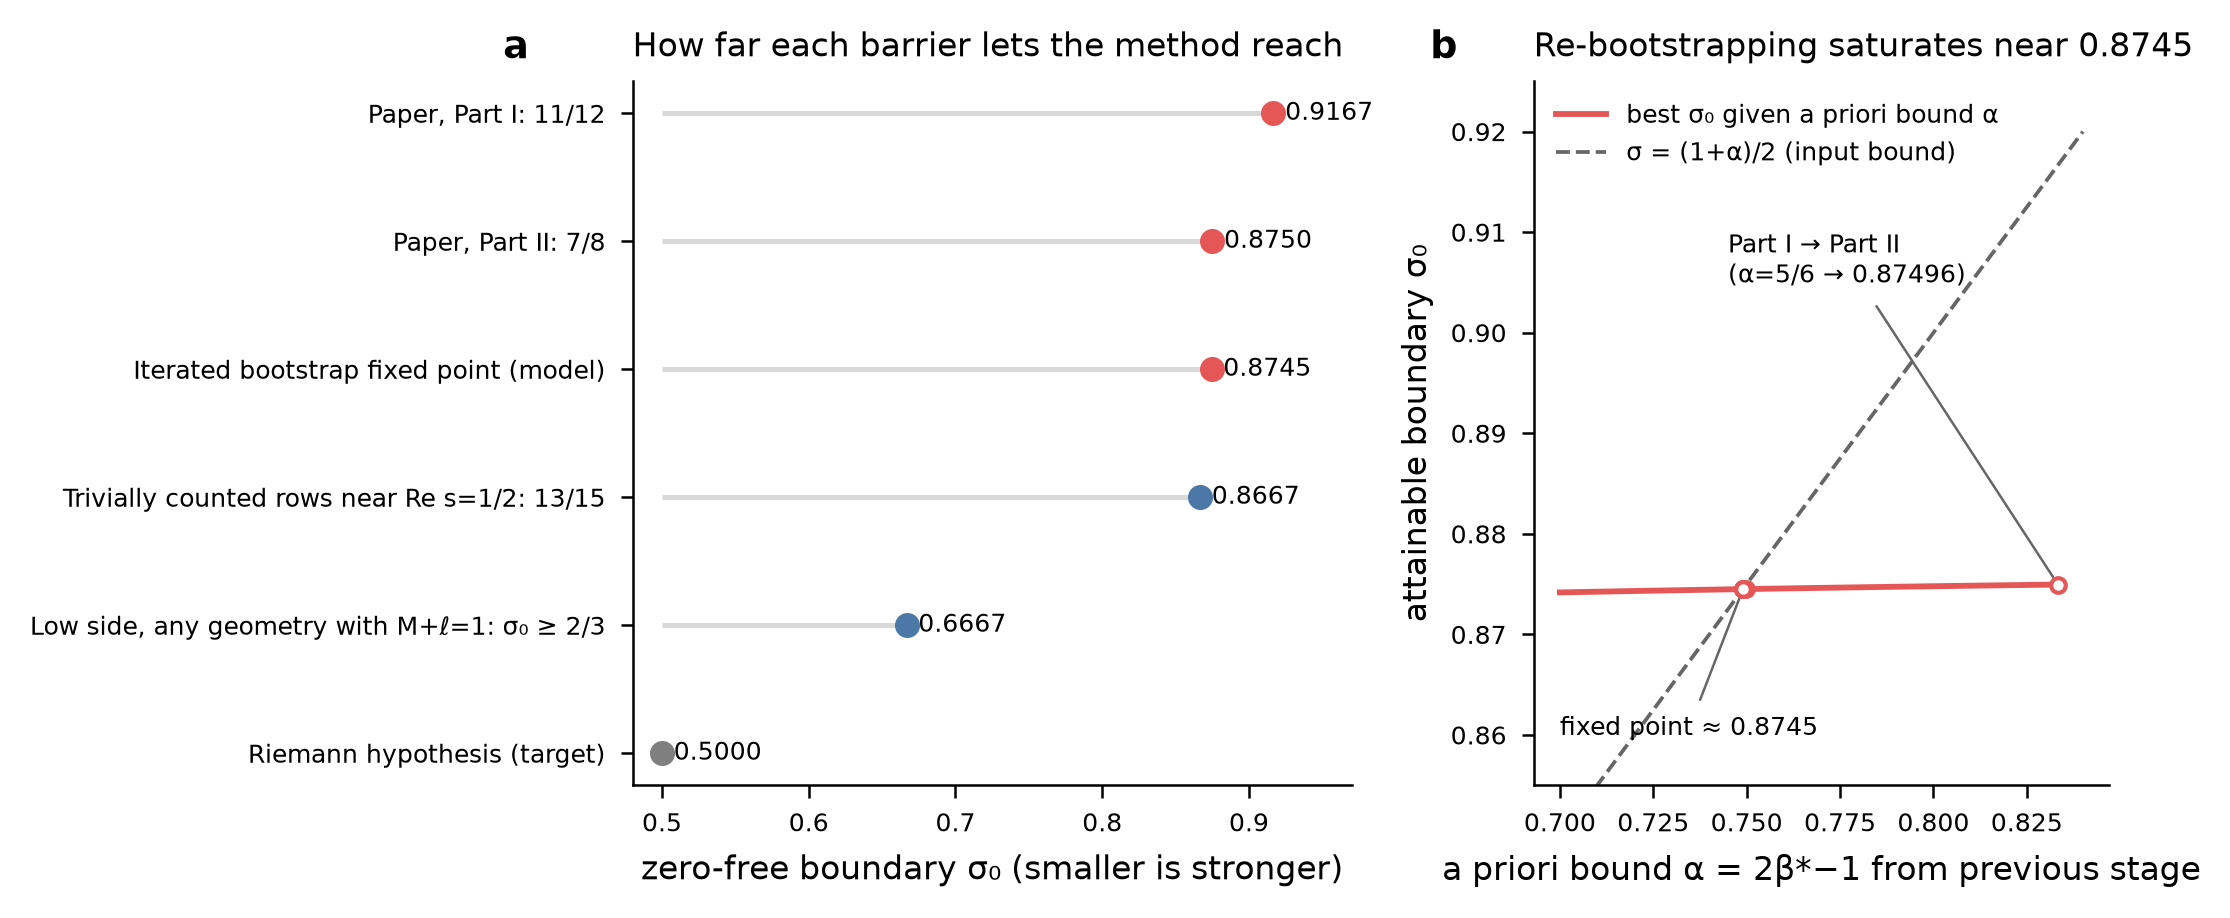
\includegraphics[width=\textwidth]{../figures/fig_barrier.png}
\caption{(a) The boundaries reachable under each barrier. (b) The best boundary as a function of the a priori
bound $\alpha=2\beta_*-1$ from the previous stage; iterating the bootstrap saturates near $0.8745$. Both
panels use the paper's exponent formulas extended verbatim beyond their stated ranges, so they give optimistic
bounds.}
\end{figure}

\section{Requests to the authors}
\begin{enumerate}
\item Provide a mapping from the paper's numbered statements to Lean declaration names, at least for
  Proposition~5.1, Lemma~9.1, Lemma~17.1, Lemma~18.1 and Proposition~19.2.
\item Publish a comparator log (including \texttt{nanoda} or \texttt{lean4checker} replay) for the three
  challenges.
\item Clarify the role of the dependency patches and of the Hecke challenge definitions.
\end{enumerate}

\section*{Limitations of this report}
This report does not replace expert peer review. A planned independent LLM-based second opinion on each lemma
could not be run because of a usage limit. The barrier and improvement analyses are model computations built
on the paper's explicit exponent formulas; they do not establish that the corresponding lemmas extend.

\begin{thebibliography}{9}
\bibitem{BIMS} A.~Bhargava, G.~Ivanyos, R.~Mittal, N.~Saxena, as cited in the preprint (not checked).
\end{thebibliography}
\end{document}
